\documentclass{article}
\usepackage[utf8]{inputenc}

\title{Error-correctie van QR-codes}
\author{Tjeu Kayim}
\date{... december 2016}
\usepackage[T1]{fontenc}
\usepackage[scaled=0.85]{beramono}
%\usepackage{bold}
\usepackage{minted}
%\usemintedstyle{tango}
\usepackage{amsmath}
\usepackage{breqn} % om lange polynomen automatisch te verdelen over verschillende regels
\usepackage{amssymb}
\usepackage{multirow}
%\usepackage{wrapfig}
\usepackage{tabto}
%\usepackage{polynom}
\usepackage{fullpage}
\usepackage{pdflscape}
\usepackage[dutch]{babel}
\usepackage{graphicx}
\graphicspath{ {images/} }
\begin{document}
\newcommand*\xor{\mathbin{\oplus}}
\def\blockms#1{\begin{minipage}{\linewidth} \texttt{#1}\end{minipage}}
\def\boldms#1{\texttt{\textbf{#1}}}
\renewcommand*\contentsname{Inhoud}
\maketitle
\newpage
\tableofcontents

\section{Inleiding}
Dit profielwerkstuk behandelt een toepassing van wiskunde voor digitale apparaten: methodes om informatie zo te coderen dat er later eventuele fouten gecorrigeerd kunnen worden door wiskundige algoritmes. Het vakgebied van wiskundige error-correctie heet coderingstheorie. Deel één gaat over de coderingstheorie in het algemeen, en wordt de Hamming-code behandelt. In het tweede deel wordt uitgelegd hoe coderingstheorie een toepassing heeft in QR-codes. Het hele proces van het maken van QR-codes wordt behandeld, inclusief de bijbehorende wiskunde en uitleg hoe dit geprogrammeerd kan worden.

In de digitale wereld van nu moet iedereen aanvaarden dat het onmogelijk is om alle techniek volledig te begrijpen. We maken vaak gebruik van erg complexe apparaten terwijl we niet precies weten hoe ze werken. Soms denken we te weten hoe iets werkt, maar blijkt het eigenlijk veel ingewikkelder te zijn. Of je denkt juist dat je nooit zal kunnen snappen hoe een bepaalde techniek werkt, en probeer je het daarom ook maar niet. Maar meestal is het best te doen om een globaal beeld te krijgen van de werking van techniek. Dat u de moeite heeft genomen dit werkstuk te lezen, betekend dat je toch een poging wilt wagen. De pagina's vol wiskunde mag je best overslaan. Maar wil je juist meer weten, kan je verder bouwen op m'n QR-code-generator. Of gebruik deze uitleg om zelf een QR-code-generator te programmeren op je eigen manier.

Dit onderwerp sprak me aan omdat het een praktische toepassing is van wiskunde. Ik ben redelijk goed met wiskunde, maar vindt het pas echt interessant als het een duidelijke toepassing krijgt. Bij dit onderwerp kon ik ook nog programmeren, wat ik best leuk vindt om te doen. Ik heb me altijd al afgevraagd hoe zo'n QR-code nu echt werkt, dus toen ik op de site van de TU in Eindhoven las hoe coderingstheorie als profielwerkstukonderwerp werd aangeraden, dacht ik: Waarom combineer ik dat niet met elkaar, en ga ik uitzoeken hoe de error-correctie van QR-codes werkt. Het bleek een stuk ingewikkelder dan ik had gedacht, maar de wiskunde viel me wel mee.

\section{Wat is de coderingstheorie?}
\subsection{Wat is het nut van coderingstheorie, wat zijn toepassingen?}
Bij elke overdracht van informatie kunnen fouten worden gemaakt. Als je met iemand praat, kan het zijn dat je de ander niet verstaat, je zou een woord verkeerd kunnen uitspreken, of de ander verstaat het verkeerd. Als je een CD afspeelt, kan het het zijn dat de speler hapert doordat er krassen op de CD zitten. Als computers digitaal informatie versturen of ontvangen, kunnen er ook fouten optreden. Vaak ontstaan die fouten door ‘ruis’.

Ruis bestaat uit willekeurige variaties in een signaal. Die variaties hebben allerlei oorzaken, bij een radio ontstaat ruis bijvoorbeeld door alle kanalen die elkaar storen, en door bepaalde sterren die radiogolfen uitzenden. Hoe krachtiger het signaal is, hoe kleiner de kans is op fouten door ruis. Digitale signalen hebben minder last van ruis dan analoge, maar er blijft altijd een kleine kans op fouten.

Soms is er maar een heel zwak signaal, bijvoorbeeld bij de communicatie met een marsrover. Door de lage signaal-ruis verhouding is de kans op fouten dan erg groot. Voor dat soort situalties zijn er technieken bedacht om fouten te corrigeren.

Toepassingen van coderingstheorie vindt je dus in CD's, bij communicatie met satellieten of ruimtesondes, bij telefonie, in QR-codes en andere vormen van digitale communicatie.
\subsection{Welke wiskundige hebben aan coderingstheorie gewerkt?}
Toen in de 20e eeuw allerlei digitale apparaten werden uitgevonden, werd het soms nodig om fouten te detecteren. In 1951 werd een enkelvoudige pariteitscontrole gebruikt om informatie op tape op te slaan. Dat werkt zo: De bits worden in groepen verdeeld, en van elke groep bepaal je de som van de bits. Is de som even, is de pariteitsbit een 0, en is het oneven, voeg je een 1 toe. Als er dan één fout optreed, klopt de partiteitsbit niet meer, en kan je zo achterhalen dat er iets verkeerd ging. Deze pariteitscontrole kan alleen niet meer dan één fout detecteren, en kan ook niet de fout corrigeren.

De simpelste manier om fouten te corrigeren, is het herhalen van elke bit. Dus de rij ‘1 0 0 1’ wordt bijvoorbeeld ‘1111 0000 0000 1111’. Deze methode maakt het bericht alleen veel langer, en is dus helemaal niet efficiënt.

De wiskundige Claude Shannon onderzocht dit probleem. Hij gaf het wiskundige bewijs dat het mogelijk was om berichten te coderen op zo'n manier dat het aantal extra bits zo klein mogelijk wordt gehouden. Hiermee legde hij de basis van de coderingstheorie.

Hij
Unfortunately his proof did not give any explicit recipes for these optimal codes.
- Richard Hamming
\subsection{Wanneer en hoe hebben de ontwikkelingen binnen de coderingstheorie plaatsgevonden?}
(wat geschiedenis)
\subsection{Welke verschillende foutcorrigerende methodes zijn er ontwikkeld en wat zijn de voordelen?}
(vergelijking van methodes)
Shannon limiet
\subsection{Hoe werkt de Hamming-code?}
(relatief eenvoudig te begrijpen, maar maakt wel duidelijk hoe wiskunde wordt toegepast, moet dit hoofdstuk nog overnemen van mijn aantekeningen)
\section{Hoe wordt de coderingstheorie toegepast in QR-codes?}
\subsection{Hoe werkt een QR-code}
Wat is een QR-code? Een zwart wit geblokt vierkantje, dat je kan scannen met je smartphone. Qr-codes worden gebruikt om informatie vast te leggen in een afbeelding, die makkelijk door een elektronisch apparaat gescant kan worden. Er zijn veel verschillende manieren om QR-codes te gebruiken, maar het bekendste is een URL: een link naar een website of applicatie. Als de code door een smartphone wordt gescand, herkent de software de QR-code, decodeert de informatie en opent de URL in een webbrowser. Er wordt gebruik gemaakt van de Reed-Solomon code als error-correctie, daardoor kan een aantal fouten worden verbeterd.

Omdat QR-codes maar een kleine hoeveelheid data bevatten, is het nog net te doen om een kleine QR-code met de hand te maken. Dat maakt het een interessant studie-object.

\subsection{Hoe wordt tekst omgezet naar bits?}
\subsubsection{UTF-8}
Het maken van QR-codes wordt meestal door computers of smartphones gedaan, omdat het een ingewikkeld en tijdrovend proces is. Toch is het proces best te begrijpen, als je er even de tijd voor neemt. We zullen nu met de hand stap voor stap een QR-code gaan coderen met de tekst “Coderingstheorie”.
Om te beginnen moet de boodschap omgezet worden van letters naar bytes, we maken daarbij gebruik van UTF-8, een onderdeel van Unicode. Hieronder is een deel van de tabel te zien om letters te coderen.\\\\
%\begin{wrapfigure}{r}{0.5\textwidth}
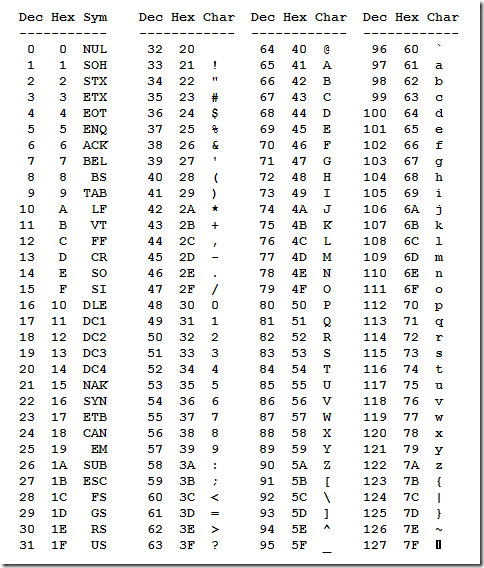
\includegraphics[width=0.4\linewidth]{unicode.png}
%\end{wrapfigure}
\subsubsection{Hexadecimaal}
In de tabel ‘Dec’ voor decimaal, de normale schrijfwijze van getallen. Daarnaast staat de Hexadecimale notatie: een talstelsel waarbij niet met tien cijfers, maar met zestien cijfers wordt geteld. De cijfers 0 t/m 9 worden uitgebreid met 'A' (10) t/m 'F' (15). De hexadecimale notatie wordt vaak gebruikt om binaire getallen kort te schrijven. Vaak worden er bytes gebruikt, acht bits, en die zijn met twee hexadecimale cijfers te schrijven. Hoe dat werkt zie je duidelijk in deze tabel:\\
%\begin{wrapfigure}{r}{0.4\textwidth}
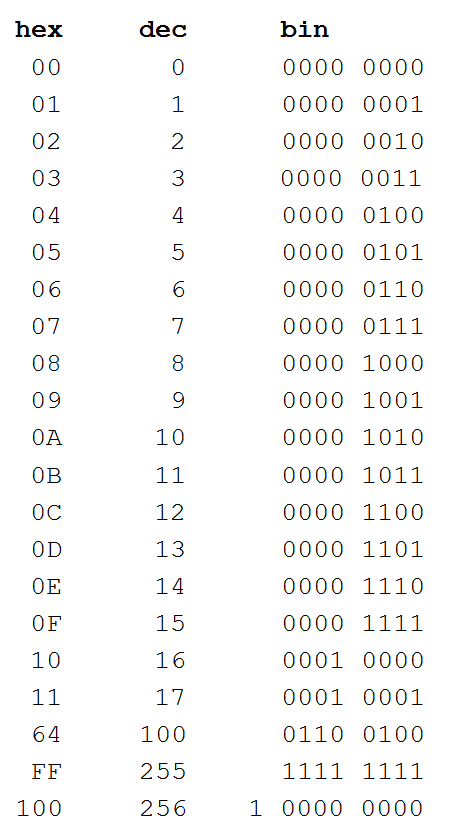
\includegraphics[width=0.3\linewidth]{hex-dec-bin-table2.png}\\
%\end{wrapfigure}
We coderen dus het woord ‘Coderingstheorie’ met UTF-8 naar hexadecimale getallen:\\\\
\texttt{
\begin{tabular}{llllllllllllllll}
C&o&d&e&r&i&n&g&s&t&h&e&o&r&i&e\\
43&6F&64&65&72&69&6E&67&73&74&68&65&6F&72&69&65\\
\end{tabular}
}\\
Dan zetten we dat om naar binair:\\\\
\blockms{01000011 011011110 11001000 11001010 11100100 11010010 11011100 11001110 11100110 11101000 11010000 11001010 11011110 11100100 110100101 100101\\}
Deze stappen worden ook uitgevoerd als je een Word document opslaat, of als je een Whatsapp berichtje verstuurd.
\subsubsection{Verder Coderen}
Er zijn verschillende groottes qr-codes, en verschillende error-correctie levels. We gebruiken de versie met de minste partiteit, zodat we het nog met de hand kunnen berekenen. Dan past het nog net in het kleinste formaat: Versie 1.
We moeten duidelijk maken dat we UTF-8 gebruiken en een ‘mode indicator’ toevoegen aan het begin: voor binary is dat \boldms{0100}. Daarna komt nog een ‘Character Count’, het aantal letters dat we coderen. In dit geval zijn dat er 16, binair geschreven \boldms{00010000}.\\\\
\blockms{\textbf{0100 00010000} 01000011 01101111 01100100 01100101 01110010 01101001 01101110 01100111 01110011 01110100 01101000 01100101 01101111 01110010 01101001 01100101\\}
Daarna wordt alles in bytes verdeeld, ofwel in groepjes van acht, en vullen we de laatste byte verder op met nullen:\\\\
\blockms{01000001 00000100 00110110 11110110 01000110 01010111 00100110 10010110 11100110 01110111 00110111 01000110 10000110 01010110 11110111 00100110 10010110 0101\textbf{0000}\\}
Er passen 19 bytes in een versie 1 QR-code, en we zitten nu op 18. De rest moet worden opgevuld met het herhalen van de bytes \boldms{11101100} en  \boldms{00010001} totdat de maximale capaciteit is bereikt, in dit geval al na het toevoegen van één byte.\\\\
\blockms{01000001 00000100 00110110 11110110 01000110 01010111 00100110 10010110 11100110 01110111 00110111 01000110 10000110 01010110 11110111 00100110 10010110 01010000 \textbf{11101100}\\}
Dat zetten we om naar de hexadecimale notatie:\\\\
\blockms{41 04 36 F6 46 57 26 96 E6 77 37 46 86 56 F7 26 96 50 EC}
Zo wordt het te coderen bericht dus omgezet naar bytes. In grotere QR-codes worden deze bytes nog gesplitst in meerdere blokken, waarvan allemaal afzonderlijk error-correctie-bytes worden berekent. Hierover later meer.
Ik heb voor het omzetten naar bytes een programma geschreven in de programmeertaal Python:
\begin{minted}{python}
# (alles waarvoor een hekje staat is uitleg)
# Definiëer een functie die tekst codeert met uft-8
def qr_encode_to_utf8(tekst,n):
    # zet tekst om in utf-8
    tekst = bytes(tekst, "utf8")
    # zet om naar bytes
    bits = ''.join(["{0:08b}".format(x) for x in tekst])
    # voeg de `mode indicator' en het aantal tekens toe
    bits = '0100' + "{0:08b}".format(len(tekst)) + bits
    # voeg nullen toe totdat een veelvoud van 8 is bereikt
    # of de maximale lengte is bereikt
    while len(bits) % 8 and len(bits) != n*8:
        bits += '0'
    # past het wel?
    if len(bits) > n*8:
        print('Het te coderen bericht is te groot voor deze versie')
        return
    # herhaal 11101100 en 00010001 totdat de maximale lengte is bereikt
    i = 0
    while len(bits) != n*8:
        if i%2: bits += '00010001'
        else: bits += '11101100'
        i += 1
    return bits
\end{minted}
\subsection{Hoe werkt de Reed-Solomoncode, en hoe wordt die hier toegepast?}
De Reed Solomon code (RS-code) is een fout-corrigerende techniek en valt onder de BCH-codes. Het wordt bijvoorbeeld gebruikt bij error-correctie van DVD's en QR-codes. Door pariteitsbits toe te voegen, kan een aantal fouten worden gecorrigeerd, net als bij de Hamming-code. Voor betere foutcorrectie is meer opslagruimte nodig door die partiteitsbits. Maar de RS-code is daarin wel erg efficiënt, en er kunnen namelijk relatief veel fouten worden gecorigeerd met weinig partiteit. \par
De komende uitleg bevat veel ingewikkelde wiskunde, maar ik zal proberen duidelijk te maken waarvoor elk stukje wiskunde nuttig is. Ik zal ook laten zien hoe ik de wiskunde heb geïmplementeerd in een programma, geschreven in Python.

\subsection*{Galoisveld}
De berekeningen bij de RS-code werken met polynomen in een $2^8$ Galoisveld. Dat is een lichaam met een eindig aantal elementen, in dit geval 0 tot en met 255. Dat zijn 256 elementen (0 telt ook mee), en zo'n Galoisveld wordt genoteerd als GF(256) of $\mathbb{F}_{256}$. Omdat de verzameling getallen eindig is, gelden er andere bewerkingen.\par
Het voordeel van dit Galoisveld is dat alle getallen precies in één byte byte passen, en dat is voor computers erg handig. Computers kunnen veel sneller en efficiënter werken als ze in zo'n Galoisveld rekenen. Alle codewoorden hebben door het Galoisveld ook een vaste lengte, waardoor het veel makkelijker gebruikt kan worden in een bepaald protocol, zoals het protocol van de QR-code.\par
Een wiskundig lichaam maakt het mogelijk om te rekenen met een begrensd aantal getallen, maar daar zijn wel speciale rekenregels voor nodig.
\subsubsection*{Optellen}
In dit lichaam moeten de bewerkingen optellen, aftrekken, vermenigvuldigen en delen allemaal gesloten zijn: de uitkomsten moeten binnen het lichaam blijven. Daarom gelden er speciale rekenregels.\par
Optellen en aftrekken staat gelijk aan de bewerking Exlusive OR (XOR). Dat is een logische poort waarbij de output 1 is als één van de bits 1 is. De wiskundige notatie van XOR is $\xor$, en in veel programmeertalen wordt het genoteerd als ^. Deze logische poort werkt zo:
$$0\xor0=0$$
$$1\xor1=0$$
$$1\xor0=1$$
$$0\xor1=1$$
Dit lijkt op optellen modulo 2:
$$0+0=0\mod{2}$$
$$1+1=0\mod{2}$$
$$1+0=1\mod{2}$$
$$0+1=1\mod{2}$$
Het optellen werkt met bits, dus moet je de getallen die je wilt optellen eerst omrekenen naar binaire getallen. Daarna zet je de getallen onder elkaar, en bereken je de som per bit. Om bijvoorbeeld $197 \xor 99$ te bereken doe je het volgende:
$$197 = 1\cdot2^7 + 1\cdot2^6 + 0\cdot2^5 + 0\cdot2^4 + 0\cdot2^3+ 1\cdot2^2 + 0\cdot2^1 + 1\cdot2^0$$
$$99 = 0\cdot2^7 + 1\cdot2^6 + 1\cdot2^5 + 0\cdot2^4 + 0\cdot2^3+ 0\cdot2^2 + 1\cdot2^1 + 1\cdot2^0$$
\\\blockms{\noindent
1 1 0 0 0 1 0 1 (197)\\
0 1 1 0 0 0 1 1 (99)\\
--------------------------- XOR\\
1 0 1 0 0 1 1 0\\
}
Dan rekenen we \texttt{10100110} weer om naar decimaal: $2^7+2^5+2^2+2^1=166$. Dus $197 \xor 99 = 166$
\subsubsection*{Vermenigvuldigen met machten van 2}
Vermenigvuldigen gaat met de rekenregel $2^a+2^b=2^{a+b}$. Alle coëfficiënten van de polynomen moeten dan dus geschreven worden als machten van twee: $2^n$, waarbij $n \in [0,255]$. Maar alle getallen moeten wel in het Galoisveld $\mathbb{F}_{256}$ blijven. Tot $n = 7$ gaat dat goed:
$$2^0=1$$
$$2^1=2$$
$$2^2=4$$
$$2^3=8$$
$$2^4=16$$
$$2^5=32$$
$$2^6=64$$
$$2^7=128$$
Maar $2^8$ is te groot voor $\mathbb{F}_{256}$, en dan moeten de getallen byte-wise modulo 100011101 genomen worden: er moet 258 vanaf getrokken worden. Dus elke bit van $2^8$ (binair 100000000) moet met 285 (binair 100011101) worden geXORed, zoals is vastgesteld in de QR-code specificaties. 285 is een irreducibele polynoom van de 8e graad. Het is niet te schrijven als het product van kleinere polynomen, en wordt ook wel een `priempolynoom' genoemd.\\\\
\blockms{100000000 (256)\\
100011101 (285)\\
--------------- XOR\\
000011101 (29)
}
\\\\
Nu kunnen we verder met de machten van 2.
$$2^8 = 29$$
$$2^9 = 2\cdot2^8 = 2\cdot29 = 58$$
$$2^{10} = 2^9 \cdot 2 = 58 \cdot 2 = 116$$
\[
\begin{array}{lll}
1&2^3
\end{array}
\]
Als exponenten groter uitkomen dan 255, bijvoorbeeld bij $2^{250}+2^{10}=2^{260}$, dan moet de exponent modulo 255 genomen worden: $2^{260}=2^{260 \mod{255}}=2^5$. Met deze methode zijn alle getallen in $\mathbb{F}_{256}$ te schrijfen als $2^n$, waarbij $n \in [0,255]$. Om verwarring met normaal machtsverheffen te voorkomen wordt $2^n$ als $\alpha^n$ geschreven. \par
Ik heb een stukje geprogrammeerd om een tabel te genereren voor de exponenten en logaritmes. Ik heb er veel uitleg bijgeschreven, zodat het duidelijk is wat het programma doet.
\begin{minted}[mathescape]{python}
# Maak een lege tabel aan voor de exponenten van 2 in het Galoisveld (gf)
gf_exp = []
# en een tabel voor de logaritmes (met 256 plaatsen)
gf_log = [0] * 256
# Deze functie vult de tabel, waarbij als argument de priempolynnoom moet worden gegeven
def tabel_exponenten(priem_polynoom):
    global gf_exp, gf_log
    x = 1
    # $2^i = x$; i is element van [0,255>
    for i in range(0,255):
        # voeg `x' ($=2^i$) toe aan de tabel voor exponenten
        gf_exp.append(x)
        # en voeg `i' toe aan de tabel voor logaritmes
        gf_log[x] = i
        # voor i+1 wordt x twee maal zo groot
        x = x*2
        # is x groter dan 255, XOR x dan met de priempolynoom
        # (XOR wordt genoteerd als ^)
        if x>255: x = x ^ priem_polynoom
# Maak een tabel met de priempolynoom 285
tabel_exponenten(285)
# De tabel wordt als volgt gebruikt
gf_exp[3] # = $2^3 = 8$
gf_log[8] # = $2\log{8} = 3$
# Vermenigvuldigen kan nu zo: $x\cdot y = \alpha^{^\alpha\!\log{x}+^\alpha\!\log{y} \mod 255}$
# want $2^a + 2^b = 2^{a+b}$
# Definiëer een functie om de argumenten x en y te vermenigvuldigen.
def gf_mul(x,y):
    # Vermenigvuldigen met 0 geeft 0
    if x==0 or y==0:
        return 0
    # modulo wordt geschreven als %
    return gf_exp[(gf_log[x]+gf_log[y]) % 255]
\end{minted}
\section*{Generatorpolynoom}
Voor coderen in de Reed-Solomon code is een generatorpolynoom nodig: de polynoom waardoor straks gedeeld gaat worden en waarvan de rest de partiteit vormt. Door de deling met deze polynoom ontstaat er een speciale wiskundige `verhouding' tussen het bericht en de partiteit, vergelijkbaar met de voorwaarden in de cirkels van de Hamming-Code. Die voorwaarden zijn nodig zodat er uiteindelijk eventuele fouten gecorrigeerd kunnen worden.\\
De generatorpolynoom voor de Reed-Solomon code is als volgt gedefinieerd:
$$g_n(x)=(x-\alpha^0)(x-\alpha^1)(x-\alpha^2) ... (x-\alpha^{n-1})$$
Waarbij $n$ het aantal fout-corrigerende codewoorden is dat moet worden gegenereerd, bij het coderen van het woord `Coderingstheorie' is $n$ gelijk aan 22.
%$$(1x-a)(1x-b)(1x-c)=$$
%$$(1x^2-ax^1-bx^1+abx^0)(1x-c)=$$
%$$(1x^2-(a+b)x^1+abx^0)(1x-c)=$$
%$$1x^3-cx^2-(a+b)x^2+c(a+b)x^1+abx^1+abcx^0=$$
%$$1x^3-(a+b+c)x^2+c(a+b)x^1+abx^1+abcx^0$$

Om de haakjes van de generatorpolynoom weg te werken, moet rekening worden gehouden met de rekenregels van het eindige lichaam waarin we werken. Optellen en aftrekken word gedaan met Exclusive OR en vermenigvuldigen van $\alpha^b$ en $\alpha^c$ geeft $\alpha^{b+c}$. De notatie met machten zal dus een aantal keer omgerekend moeten worden naar bits, en andersom. Ik zal een beginnen met het berekenen van een generatorpolynoom voor twee error-correctie codewoorden.
$$g_2(x)=$$
$$(\alpha^0x - \alpha^0) \cdot (\alpha^0x - \alpha^1)=$$
$$(\alpha^0x^1 \cdot \alpha^0x^1) + (\alpha^0x^0 \cdot \alpha^0x^1) + (\alpha^0x^1 \cdot \alpha^1x^0) + (\alpha^0x^0 \cdot \alpha^1x^0)$$
Bij vermenigvuldigen de exponenten optellen:
$$(\alpha^{0+0}x^{1+1}) + (\alpha^{0+0}x^{0+1}) + (\alpha^{0+1}x^{1+0}) + (\alpha^{0+1}x^{0+0})=$$
$$\alpha^0x^2 + \alpha^0x^1 + \alpha^1x^1 + \alpha^1x^0=$$
$$\alpha^0x^2 + (\alpha^0+\alpha^1)x^1 + \alpha^1x^0$$
Optellen wordt gedaan met Exclusive OR.
$$x^2 + (1\xor2)x^1 + 2x^0$$
\blockms{01 (1)\\
10 (2)\\
------ XOR\\
11 (3)
}
$$x^2 + 3x^1 + 2x^0$$
Dan omrekenen naar de notatie met machten van alpha.
$$\alpha^0x^2 + \alpha^{25}x^1 + \alpha^1x^0$$
Dit is dus de generatorpolynoom voor twee codewoorden. Vermenigvuldigen we dat met $(x-\alpha^2)$, dan krijgen we $g_3(x)$.
$$g_3(x)=$$
$$(\alpha^0x^2 + \alpha^{25}x^1 + \alpha^1x^0) \cdot (\alpha^0x^1 + \alpha^2x^0)=$$
$$\alpha^0x^2 \cdot \alpha^0x^1 + \alpha^{25}x^1 \cdot \alpha^0x^1 + \alpha^1x^0 \cdot \alpha^0x^1 + \alpha^0x^2 \cdot \alpha^2x^0 + \alpha^25x^1 \cdot \alpha^2x^0 + \alpha^1x^0 \cdot \alpha^2x^0=$$
$$\alpha^{0+0}x^{2+1} + \alpha^{25+0}x^{1+1} + \alpha^{1+0}x^{0+1} + \alpha^{0+2}x^{2+0} + \alpha^{25+2}x^{1+0} + \alpha^{1+2}x^{0+0}=$$
$$\alpha^0x^3 + \alpha^{25}x^2 + \alpha^1x^1 + \alpha^2x^2 + \alpha^{27}x^1 + \alpha^3x^0=$$
$$\alpha^0x^3 + (\alpha^{25} \xor \alpha^2)x^2 + (\alpha^1 \xor \alpha^{27})x^1 + \alpha^3x^0=$$
$$\alpha^0x^3 + (3 \xor 4)x^2 + (2 \xor 12)x^1 + \alpha^3x^0=$$
\\
\blockms{011 (3)\\
100 (4)\\
--------- XOR\\
111 (7)\\
}
\blockms{1100 (12)\\
0010 (2)\\
--------- XOR\\
1110 (14)\\
}
$$\alpha^0x^3 + 7x^2 + 14x^1 + \alpha^3x^0=$$
$$\alpha^0x^3 + \alpha^{198}x^2 + \alpha^{199}x^1 + \alpha^3x^0$$
Voor $g_4(x)$ vermenigvuldigen we dat met $(x-\alpha^3)$:
$$g_4(x)=$$
\begin{dmath*}(\alpha^{0}x^{3}+\alpha^{198}x^{2}+\alpha^{199}x+\alpha^{3})(\alpha^{0}x+\alpha^{3})=\end{dmath*}
\begin{dmath*}\alpha^{0+0}x^{3+1}+\alpha^{0+198}x^{2+1}+\alpha^{0+199}x^{1+1}+\alpha^{0+3}x^{0+1}+\alpha^{3+0}x^{3+0}+\alpha^{3+198}x^{2+0}+\alpha^{3+199}x^{1+0}+\alpha^{3+3}=\end{dmath*}
\begin{dmath*}\alpha^{0}x^{3}+\alpha^{198}x^{2}+\alpha^{199}x^{1}+\alpha^{3}x^{0}+\alpha^{3}x^{4}+\alpha^{201}x^{3}+\alpha^{202}x^{2}+\alpha^{6}=\end{dmath*}
$$\alpha^{0}x^{4}+\alpha^{75}x^{3}+\alpha^{249}x^{2}+\alpha^{78}x+\alpha^{6}$$
$$g_5(x)=$$
\begin{dmath*}(\alpha^{0}x^{4}+\alpha^{75}x^{3}+\alpha^{249}x^{2}+\alpha^{78}x+\alpha^{6})(\alpha^{0}x+\alpha^{4})=\end{dmath*}
\begin{dmath*}\alpha^{0+0}x^{4+1}+\alpha^{0+75}x^{3+1}+\alpha^{0+249}x^{2+1}+\alpha^{0+78}x^{1+1}+\alpha^{0+6}x^{0+1}+\alpha^{4+0}x^{4+0}+\alpha^{4+75}x^{3+0}+\alpha^{4+249}x^{2+0}+\alpha^{4+78}x^{1+0}+\alpha^{4+6}=\end{dmath*}
\begin{dmath*}\alpha^{0}x^{4}+\alpha^{75}x^{3}+\alpha^{249}x^{2}+\alpha^{78}x^{1}+\alpha^{6}x^{0}+\alpha^{4}x^{5}+\alpha^{79}x^{4}+\alpha^{253}x^{3}+\alpha^{82}x^{2}+\alpha^{10}=\end{dmath*}
$$\alpha^{0}x^{5}+\alpha^{113}x^{4}+\alpha^{164}x^{3}+\alpha^{166}x^{2}+\alpha^{119}x+\alpha^{10}$$
$$g_6(x)=$$
\begin{dmath*}(\alpha^{0}x^{5}+\alpha^{113}x^{4}+\alpha^{164}x^{3}+\alpha^{166}x^{2}+\alpha^{119}x+\alpha^{10})(\alpha^{0}x+\alpha^{5})=\end{dmath*}
\begin{dmath*}\alpha^{0+0}x^{5+1}+\alpha^{0+113}x^{4+1}+\alpha^{0+164}x^{3+1}+\alpha^{0+166}x^{2+1}+\alpha^{0+119}x^{1+1}+\alpha^{0+10}x^{0+1}+\alpha^{5+0}x^{5+0}+\alpha^{5+113}x^{4+0}+\alpha^{5+164}x^{3+0}+\alpha^{5+166}x^{2+0}+\alpha^{5+119}x^{1+0}+\alpha^{5+10}=\end{dmath*}
\begin{dmath*}\alpha^{0}x^{5}+\alpha^{113}x^{4}+\alpha^{164}x^{3}+\alpha^{166}x^{2}+\alpha^{119}x^{1}+\alpha^{10}x^{0}+\alpha^{5}x^{6}+\alpha^{118}x^{5}+\alpha^{169}x^{4}+\alpha^{171}x^{3}+\alpha^{124}x^{2}+\alpha^{15}=\end{dmath*}
$$\alpha^{0}x^{6}+\alpha^{166}x^{5}+\alpha^{0}x^{4}+\alpha^{134}x^{3}+\alpha^{5}x^{2}+\alpha^{176}x+\alpha^{15}$$
$$g_7(x)=$$
\begin{dmath*}(\alpha^{0}x^{6}+\alpha^{166}x^{5}+\alpha^{0}x^{4}+\alpha^{134}x^{3}+\alpha^{5}x^{2}+\alpha^{176}x+\alpha^{15})(\alpha^{0}x+\alpha^{6})=\end{dmath*}
\begin{dmath*}\alpha^{0+0}x^{6+1}+\alpha^{0+166}x^{5+1}+\alpha^{0+0}x^{4+1}+\alpha^{0+134}x^{3+1}+\alpha^{0+5}x^{2+1}+\alpha^{0+176}x^{1+1}+\alpha^{0+15}x^{0+1}+\alpha^{6+0}x^{6+0}+\alpha^{6+166}x^{5+0}+\alpha^{6+0}x^{4+0}+\alpha^{6+134}x^{3+0}+\alpha^{6+5}x^{2+0}+\alpha^{6+176}x^{1+0}+\alpha^{6+15}=\end{dmath*}
\begin{dmath*}\alpha^{0}x^{6}+\alpha^{166}x^{5}+\alpha^{0}x^{4}+\alpha^{134}x^{3}+\alpha^{5}x^{2}+\alpha^{176}x^{1}+\alpha^{15}x^{0}+\alpha^{6}x^{7}+\alpha^{172}x^{6}+\alpha^{6}x^{5}+\alpha^{140}x^{4}+\alpha^{11}x^{3}+\alpha^{182}x^{2}+\alpha^{21}=\end{dmath*}
$$\alpha^{0}x^{7}+\alpha^{87}x^{6}+\alpha^{229}x^{5}+\alpha^{146}x^{4}+\alpha^{149}x^{3}+\alpha^{238}x^{2}+\alpha^{102}x+\alpha^{21}$$
Na deze twee bladzijdes wiskunde, weer wat programmeren. Om het woord `Coderingstheorie' te coderen hadden we $g_7(x)$ nodig. Om dat allemaal met de hand te doen, is erg langdradig, foutgevoelig en verschrikkelijk veel werk. Ik zal dus het maken van een generatorpolynoom ook aan het programma toevoegen. Eerst moet gedefinieerd worden hoe polynomen vermenigvuldigd  worden.
\begin{minted}{python}
# Polynomen vermenigvuldigen in een Galoisveld
# polynomen worden geschreven als een 'list' met coöficiënten
# x^2 + 3x - 6 => [1,3,-6]
def gf_poly_mul(p,q):
    # r(x) = p(x) * q(x)
    # de lengte van r(x) is gelijk aan de som van de lengtes van p(x) en q(x) min 1
    r = [0] * (len(p)+len(q)-1)
    for j in range(0, len(q)):
        for i in range(0, len(p)):
        	# Voor elke term in p(x), ga alle termen in q(x) af
            # en tel het product van de te termen uit p(x) en q(x)
            # op bij de term van r(x), waarvan de exponent de som
            # is van de exponenten in de vermenigvuldigde termen
            # '^=' betekent: XOR dit met...
            r[i+j] ^= gf_mul(p[i], q[j])
            # Dit is zo'n voorbeeld waarbij de code een stuk simpeler is
            # dan de Nederlandse `uitleg'
    return r

# Maak een Reed-Solomon (rs) generatorpolynoom
# voor een bepaald aantal error-correctie codewoorden (n)
def rs_generator_poly(n):
    # g(x) = 1
    g = [1]
    # g(x) = 1*(x-alpha^0)*(x-alpha^1) ... *(x-alpha^n-1)
    for i in range(0,n):
        g = gf_poly_mul(g, [1, gf_exp[i]])
    return g
\end{minted}
\subsubsection{Synthetic Division}
In de volgende stap moeten de berichtpolynomen allebei gedeeld worden door de generatorpolynoom. Hiervoor gebruiken we de techniek `synthetische deling' of `extended synthetic division': een alternatief voor de staartdeling. Ik zal een korte uitleg geven. Stel je wilt deze deling oplossen:
$$\frac{
3x^4+200x^3+144x^2+250x+96
}{
1x^2 + 3x^1 + 2
}$$
Dat kan met een normale staartdeling voor polynomen, houdt er alleen rekening mee dat vermenigvuldigen met de alphanotatie moet, en aftrekken met Exclusive OR.
\[
\renewcommand\arraystretch{1.2}
\begin{array}{rrrrrrrr}
x^2+3x+2\text{ /} & 3x^4 & 200x^3 & 144x^2 & 250x & 96 & \text{\textbackslash} & 3x^2+205x+220\\
&3x^4 & 5x^3 & 6x^2 & \multicolumn{1}{l}{\xor}\\\cline{2-4}
&&205x^3 & 150x^2 & 250x\\
&&205x^3 & 74x^2 & 135x & \multicolumn{1}{l}{\xor} \\\cline{3-5}
&&&220x^2 & 125x & 96\\
&&&220x^2 & 121x & 165 & \multicolumn{1}{l}{\xor} \\\cline{4-6}
&&&&4x & 197
\end{array}
\]
Deze deling kan ook gedaan worden met de `Extended Synthetic division'. Deze methode werkt alleen als de eerste coëfficiënt van de noemer gelijk is aan één. Bij de generatorpolynomen, waardoor uiteindelijk gedeeld moet worden, is dat altijd het geval.

Eerst schrijf je de coëfficiënten op van de teller, beginnend bij de grootste exponent van $x$. De coëfficiënten van de noemer schrijf je in een schuine lijn naar boven op, behalve de eerste:
\[\begin{array}{rr|rrrrr}
&&3&200&144&250&96\\
&2\\
3&&
\end{array}\]
Daarna teken je onderaan een horizontale lijn, en breng je de het eerste getal bovenaan naar beneden:
\[\begin{array}{rr|rrrrr}
&&3&200&144&250&96\\
&2\\
3&&\\\cline{3-7}
&&3
\end{array}\]
Je vermenigvuldigt de drie met de coëfficiënten van de noemer. En schrijft de producten diagonaal op. In dit Galoisveld geld $3\cdot3=5$ en $3\cdot2=6$.
\[\begin{array}{rr|rrrrr}
&&3&200&144&250&96\\
&2&&&6\\
3&&&5\\\cline{3-7}
&&3
\end{array}\]
Dan bereken je de som in de volgende kolom en schrijft die onderaan op. Optellen werkt met Exlusive OR, en in dit geval komt er toevallig hetzelfde uit als bij normaal rekenen.
\[\begin{array}{rr|rrrrr}
&&3&200&144&250&96\\
&2&&&6\\
3&&&5\\\cline{3-7}
&&3&205
\end{array}\]
Het product van 205 met 3 en 2 schrijf je weer diagonaal op.
\[\begin{array}{rr|rrrrr}
&&3&200&144&250&96\\
&2&&&6&135\\
3&&&5&74\\\cline{3-7}
&&3&205
\end{array}\]
Herhaal deze stapen totdat de diagonaal niet meer zou passen. En schrijf de som van de laatste kolommen eronder.
\[\begin{array}{rr|rrrrr}
&&3&200&144&250&96\\
&2&&&6&135&165\\
3&&&5&74&122\\\cline{3-7}
&&3&205&220&4&197
\end{array}\]
De onderste regel zijn het quotiënt en de rest. Zet een streepje zodat het aantal getallen rechts van het streepje gelijk is aan het aantal getallen links van de verticale lijn. Het streepje scheidt nu het quotiënt en de rest van elkaar.
\[\begin{array}{rr|rrrrr}
&&3&200&144&250&96\\
&2&&&6&135&165\\
3&&&5&74&122\\\cline{3-7}
&&3&205&\multicolumn{1}{r|}{220}&4&197
\end{array}\]
$$\frac{
3x^4+200x^3+144x^2+250x+96
}{
1x^2 + 3x^1 + 2
} = 3x^2 + 205x^1 + 220 + \frac{4x+197}{1x^2 + 3x^1 + 2}
$$
Deze methode is een stuk systematischer, en daardoor makkelijker te programmeren.
\begin{minted}{python}
def poly_div(self,teller, noemer):
    '''Synthethic Division (Synthetische Deling)'''
    output = list(teller)
    # Voor alle diagonalen die passen
    for i in range(0, len(teller) - (len(noemer)-1)):
        # stop als de factor nul is, want log(0) bestaat niet
        if output[i] != 0:
            # de eerste coöficiënt van de noemer wordt overgeslagen
            for j in range(1, len(noemer)):
                 # stop als de factor nul is
                if noemer[j] != 0:
                    # vermenigvuldig en tel op (XOR) bij het getal onderaan de kolom
                    output[i+j] ^= self.mul(noemer[j], output[i])
    # bepaal de positie van van het verticale streepje
    # tussen het quotiënt en de teller
    streepje = -(len(noemer)-1)
    # en geef als resultaat het quotiënt en de rest
    return output[:streepje], output[streepje:]
\end{minted}
Polynomen worden hier voorgesteld als een lijst coëfficiënten tussen vierkante haken: $1x^2 + 3x^1 + 2$ wordt \texttt{[1,3,2]}. Om alle functies (vermenigvuldigen, delen, enz.) samen te brengen, defiëren we een `class'. Het eindresultaat van dit hoofdstuk is deze class, die we later zullen gebruiken bij coderen met de RS-code:
\begin{minted}{python}
class GaloisField:
    def __init__ (self,priem_poly):
        self.exp = []
        self.log = [0] * 256
        self.tabel_exponenten(priem_poly)
    def tabel_exponenten(self,priem_poly):
        x = 1
        for i in range(0,255):
            self.exp.append(x)
            self.log[x] = i
            x = x*2
            if x>255: x = x ^ priem_poly
    def mul(self,x,y):
        if x==0 or y==0:
                return 0
        return self.exp[(self.log[x]+self.log[y]) % 255]
    def poly_mul(self,p,q):
        '''Polynomen vermenigvuldigen in een Galoisveld'''
        r = [0] * (len(p)+len(q)-1)
        for j in range(0, len(q)):
            for i in range(0, len(p)):
                r[i+j] ^= gf.mul(p[i], q[j])
        return r
    def poly_div(self,teller, noemer):
        '''Synthetische Deling'''
        output = list(teller)
        for i in range(0, len(teller) - (len(noemer)-1)):
            if output[i] != 0: # log(0) bestaat niet
                for j in range(1, len(noemer)):
                    if noemer[j] != 0: # log(0) bestaat niet
                        output[i+j] ^= self.mul(noemer[j], output[i])
        streepje = -(len(noemer)-1)
        return output[:streepje], output[streepje:]


''' Gebruik '''
# Maak eerst een nieuwe instantie, met priempolynoom 285
>>> gf = GaloisField(priem_poly=285)
# Nu kunnen we zo bijvoorbeeld polynomen delen
>>> gf.poly_div([3,200,144,250,96],[1,3,2])
([3,205,220],[4,197])
\end{minted}


\begin{landscape}
\subsubsection{Coderen met de RS-code}
Het te coderen bericht moet als een polynoom geschreven worden. In het vorige hoofdstuk eindigde we met deze bytes:\\\\
\blockms{Hexadecimaal: 41 04 36 F6 46 57 26 96 E6 77 37 46 86 56 F7 26 96 50 EC\\
Decimaal: 65 4 54 246 70 87 38 150 230 119 55 70 134 86 247 38 150 80 236\\
}
We maken een 1-L versie QR-code, en die heeft volgens de specificaties 7 error-correctie codewoorden (e.c.-codewoorden). Het binaire bericht kan worden geschreven als een polynoom (de berichtpolynoom), beginnend met de hoogste macht van $x$. De laagste macht moet gelijk zijn aan het aantal e.c.-codewoorden.
\begin{dmath*}
65x^{25} + 4x^{24} + 54x^{23} + 246x^{22} + 70x^{21} + 87x^{20} + 38x^{19} + 150x^{18} + 230x^{17} + 119x^{16} + 55x^{15} + 70x^{14} + 134x^{13} + 86x^{12} + 247x^{11} + 38x^{10} + 150x^{9} + 80x^{8} + 236x^{7}
\end{dmath*}
De generatorpolynoom voor $n=7$ was dit:
$$g_7(x) = \alpha^{0}x^{7}+\alpha^{87}x^{6}+\alpha^{229}x^{5}+\alpha^{146}x^{4}+\alpha^{149}x^{3}+\alpha^{238}x^{2}+\alpha^{102}x+\alpha^{21}=x^{7} + 127x^{6} + 122x^{5} + 154x^{4} + 164x^{3} + 11x^{2} + 68x^{1} + 117$$
Om de QR-code verder te coderen, moeten we de berichtpolynoom delen door de generatorpolynoom, ik zal voor het gemak overal de normale notatie van coëfficiënten gebruiken, i.p.v de alphanotatie.
\begin{equation*}
\resizebox{\hsize}{!}{$\frac{
65x^{25} + 4x^{24} + 54x^{23} + 246x^{22} + 70x^{21} + 87x^{20} + 38x^{19} + 150x^{18} + 230x^{17} + 119x^{16} + 55x^{15} + 70x^{14} + 134x^{13} + 86x^{12} + 247x^{11} + 38x^{10} + 150x^{9} + 80x^{8} + 236x^{7}
}{
x^{7} + 127x^{6} + 122x^{5} + 154x^{4} + 164x^{3} + 11x^{2} + 68x^{1} + 117
}
$}
\end{equation*}
\textbf{Synthetische deling:}
\[
\renewcommand\tabcolsep{1.5pt}
\begin{tabular}{rrrrrrr|rrrrrrrrrrrrrrrrrrrrrrrrrr}
&&&&&&&65&4&54&246&70&87&38&150&230&119&55&70&134&86&247&38&150&80&236&0&0&0&0&0&0&0\\
&&&&&&117&&&&&&&&121&39&115&245&156&17&153&177&193&82&6&81&217&24&1&157&232&62&218\\
&&&&&68&&&&&&&&148&62&44&186&248&49&164&126&102&122&104&78&219&189&231&31&91&100&239&\\
&&&&11&&&&&&&&241&108&118&25&173&222&96&70&128&103&125&215&105&233&155&54&61&30&217&&\\
&&&164&&&&&&&&214&209&157&13&99&61&200&249&246&117&57&231&18&228&133&230&66&176&128&&&\\
&&154&&&&&&&&211&183&48&34&230&36&25&178&215&45&170&120&69&146&51&213&79&22&16&&&&\\
&122&&&&&&&&145&88&129&149&125&40&117&53&71&34&251&209&140&203&81&44&86&194&127&&&&&\\
127&&&&&&&&201&134&36&181&34&63&218&73&206&249&91&90&191&113&97&67&60&150&28&&&&&&\\\cline{8-33}
&&&&&&&65&205&33&89&19&240&35&190&143&204&32&220&15&128&251&232&233&182&\multicolumn{1}{r|}{31}&136&226&131&88&85&209&218
\end{tabular}\]
Reken de rest van de deling om naar om naar bits, en voeg het toe aan de bits van het bericht:\\\\
\blockms{01000001 00000100 00110110 11110110 01000110 01010111 00100110 10010110 11100110 01110111 00110111 01000110
10000110 01010110 11110111 00100110 10010110 01010000 11101100 \textbf{10001000 11100010 10000011 01011000 01010101 11010001 11011010}}
\end{landscape}
\noindent
Deze stappen kunnen we ook toevoegen aan het programma:
\begin{minted}{python}
def rs_encode(msg_in,ec):
    ''' Codeer een bepaalde berichtpolynoom met de RS-code; ec is het aantal e.c.-codewoorden '''
    # Bereken de generatorpolynoom
    generator = rs_generator_poly(ec)
    # Laat de machten van de berichtpolynoom beginnen bij het aantal e.c-codewoorden
    # en deel het door de generatorpolynoom
    quotient, rest = gf.poly_div(msg_in + [0] * ec, generator)
    # Voeg de rest van de deling toe aan de databytes en return dat
    return msg_in, rest
>>> rs_encode(
    [ 65, 4, 54, 246, 70, 87, 38, 150, 230, 119, 55, 70, 134, 86, 247, 38, 150, 80, 236]
    ,ec = 7)
[65, 4, 54, 246, 70, 87, 38, 150, 230, 119, 55, 70, 134, 86, 247, 38, 150, 80, 236, 81, 80,
81, 80, 81, 129, 64]
*** Controleren ***
\end{minted}

\subsection{Hoe bouw je een QR-code?}
\subsubsection{Aantal blokken \& e.c-bytes}
Grotere versies QR-codes bestaan uit meerdere `blokken' die allemaal afzonderlijk gecodeerd moeten worden met de RS-code. De databytes worden gesplitst in even grote blokken, met uitzondering van de 5-Q en 5-H QR-code. In de QR-code specificaties worden 40 versies beschreven, met allemaal andere groottes. Bij elk versienummer zijn 4 verschillende niveaus van error-correctie: Low, Medium, Quartile en High. `L' kan tot 7\% fouten corrigeren en `H' tot 30\%. Een aantal kleinere QR-codes kan ook nog een extra aantal fouten detecteren, maar niet corrigeren. Een 2-H QR-code heeft grootte twee en e.c-level H (High), die kan dus meer fouten corrigeren, maar de data-capaciteit neemt wel af, er passen dus minder letters in dan in bijvoorbeeld een 2-L QR-code.
Bij het coderen van `Coderingstheorie' coderen we een 1-L QR-code, die heeft dus versienummer 1 en e.c-level L. Om te weten hoe groot de bloklengte is en het aantal e.c-bytes, moet je dat opzoeken in een tabel uit de QR-code specificaties.
De eerste kolom bevat de versienummers, de tweede kolom het totaal totaal aantal bytes, dus de som van de data-bytes en de e.c-bytes. Het aantal e.c-bytes is het totaal en moet verdeeld worden over de blokken.

\[
\begin{tabular}{|c|c|c|c|c|}
\hline
\bfseries Versienummer & \bfseries Totaal aantal bytes & \bfseries E.C-level & \bfseries Aantal e.c-bytes & \bfseries Aantal blokken\\\hline
\multirow{4}{*}{1} & \multirow{4}{*}{26} &
L & 7  & 1\\&&
M & 10 & 1\\&&
Q & 13 & 1\\&&
H & 17 & 1\\\hline
\multirow{4}{*}{2} & \multirow{4}{*}{44} &
L & 10 & 1\\&&
M & 16 & 1\\&&
Q & 22 & 1\\&&
H & 28 & 1\\\hline
\multirow{4}{*}{3} & \multirow{4}{*}{70} &
L & 15 & 1\\&&
M & 26 & 1\\&&
Q & 36 & 2\\&&
H & 44 & 2\\\hline
\multirow{4}{*}{4} & \multirow{4}{*}{100} &
L & 20 & 1\\&&
M & 36 & 2\\&&
Q & 52 & 2\\&&
H & 64 & 4\\\hline
\multirow{4}{*}{5} & \multirow{4}{*}{134} &
L & 26 & 1\\&&
M & 48 & 2\\&&
Q & 72 & 2\\&&
H & 88 & 2\\\hline
\multirow{4}{*}{6} & \multirow{4}{*}{172} &
L & 36 & 2\\&&
M & 64 & 4\\&&
Q & 96 & 4\\&&
H & 112& 4\\\hline
\end{tabular}
\]
Het berekenen van het aantal data-bytes en e.c-bytes per blok moet worden toegevoegd aan het programma. Daarbij moet de tabel gedefinieerd worden in de vorm van een `two-dimensional array'. Om van alle code één geheel te maken, zal ik eerst een Class definiëren.
\begin{minted}{python}
class Qr_code:
    '''QR Code generator'''
    # Initialiseer bewerkingen Galoisveld met de priempolynoom 285
    global gf
    gf = GF(285)
    def __init__(self,bericht,versie=1,mask=0,ec='H'):
        # Controleer of de arguments geldig zijn
        if versie not in range(1,7):
            raise ValueError('Het versienummer moet tussen 1 en 6 liggen')
        if ec not in ('L','M','Q','H'):
            raise ValueError("De e.c-level moet L, M, Q of H zijn")
        if type(bericht) is not str:
            raise ValueError("Het bericht moet een 'string' zijn")
        if mask not in range(8):
            raise ValueError('mask moet tussen 1 en 7 liggen')
        while True:
            print('Genereer QR-code versie %i-%s' % (versie,ec))
            # Definiëer variables in huidige `Class'
            self.versie = versie
            self.v = versie-1
            self.grootte = self.v*4+21
            self.mask = mask
            self.ec = ec
            # Initialiseer een lege matrix met Numpy
            self.matrix = -np.ones((self.grootte,self.grootte),dtype=np.int)
            # Haal versie informatie op uit de tabel (two-demensional dictionary)
            info = __class__.versie_info[versie]
            total = info['total']
            msg_len = total - info[ec][0]
            aantal_blocks = info[ec][1]
            # codeer tekst naar bits met uft8
            try:
                self.blocks_bytes = self.encode_to_utf8(bericht,msg_len,aantal_blocks)
            except ValueError as err:
                # Is het bericht te lang:
                print(err)
                if self.versie == 6:
                    # is het versienummer 6, stop dan
                    return
                # vergroot het versienummer en probeer opnieuw of het past
                versie += 1
                continue
            # Als het bericht past, ga dan verder
            break
        ec = int(info[ec][0] / aantal_blocks)
        # codeer de blocks met de RS-code
        self.blocks_ec_bytes = [self.rs_encode(block,ec,True) for block in self.blocks_bytes]
        # combineer de data-bytes met de e.c.-bytes tot een string van bits
        qr_bits = self.interleave_blocks(rest = msg_len % aantal_blocks)
        self.voeg_finder_en_timing_patterns_toe()
        self.vul_qr_code(qr_bits)
        self.voeg_format_string_toe()
    # Versie info
    # total: totaal aantal bytes
    # (Aantal E.C-codewoorden, Aantal blocks)
    versie_info = {
        1 : {
            'total' : 26,
            'L' : (7,1),
            'M' : (10,1),
            'Q' : (13,1),
            'H' : (17,1),
        },
        ...
        6 : {
            'total' : 172,
            'L' : (36,2),
            'M' : (64,4),
            'Q' : (96,4),
            'H' : (112,4),
        }
    }
    @staticmethod
    def encode_to_utf8(tekst,n,aantal_blocks):
        # zet tekst om in utf-8
        tekst = bytes(tekst, "utf8")
        # zet om naar bytes
        bits = ''.join(["{0:08b}".format(x) for x in tekst])
        # voeg de 'mode indicator' en het aantal tekens toe
        bits = '0100' + "{0:08b}".format(len(tekst)) + bits
        # voeg nullen toe totdat een veelvoud van 8 is bereikt
        # of de maximale lengte is bereikt
        while len(bits) % 8 and len(bits) != n*8:
            bits += '0'
        # past het wel?
        if len(bits) > n*8:
            raise ValueError('Het te coderen bericht is te groot voor de opgegeven versie')
        # herhaal 11101100 en 00010001 totdat de maximale lengte is bereikt
        i = 0
        while len(bits) != n*8:
            if i%2: bits += '00010001'
            else: bits += '11101100'
            i += 1
        # splits in bytes
        bytes_list = [int(bits[i:i+8],2) for i in range(0, len(bits), 8)]
        # deel lengte door het aantal blocks
        q = len(bytes_list)/aantal_blocks
        # rond qotiënt af naar beneden
        n = int(q)
        # is er een rest?
        rest = not q == n
        # splits data-bytes in meerdere blokken
        blocks = []
        x = 0
        for i in range(aantal_blocks):
            blocks.append(bytes_list[x:x+n])
            x += n
            # als er een rest is, tel halverwege 1 bij n op
            if(rest and i==1): n += 1
        return blocks
    @classmethod
    def rs_encode(cls,msg_in,ec,return_only_ec_bytes=False):
        generator = cls.rs_generator_poly(ec)
        # Maak een berichtpolynoom met als laagste macht het aantal e.c.-codewoorden
        # en deel dit door de generatorpolynnoom
        quotient, rest = gf.poly_div(msg_in + [0] * ec, generator)
        # Return de codewoorden
        if return_only_ec_bytes:
            return rest
        else:
            return msg_in + rest
    @staticmethod
    def rs_generator_poly(n):
        # g(x)=1
        g = [1]
        # g(x)=1*(x-alpha^0)*(x-alpha^1) ... *(x-alpha^n-1)
        for i in range(0,n):
            g = gf.poly_mul(g, [1, gf.exp[i]])
        return g
    def interleave_blocks(self,rest):
        blocks = self.blocks_bytes
        ec_blocks = self.blocks_ec_bytes
        qr_bits = ''
        # loop alle kolommen af van de `message codewords' onder elkaar
        for i in range(len(blocks[0])):
            # voeg de `message codewords' toe
            for msg_bytes in blocks:
                qr_bits += "{0:08b}".format(msg_bytes[i])
        # als de laatste rijen langer zijn (bij 5-Q en 5-H)
        if rest:
            for i in (2,3):
                qr_bits += "{0:08b}".format(blocks[i][-1])
        # loop alle kolommen af van de error-correctie codewoorden onder elkaar
        for i in range(len(ec_blocks[0])):
            # voeg de e.c-codewoorden toe
            for ec_bytes in ec_blocks:
                qr_bits += "{0:08b}".format(ec_bytes[i])
        return qr_bits
\end{minted}
\subsubsection{Opbouw QR-code}
Uiteindelijk hebben we dus een string van bits gemaakt, die in de QR-code geplaatst moeten worden. Eerst moeten de drie kenmerkende vierkantjes, `finding-patterns',  geplaatst worden in de hoeken, en de `timing-patterns' (stippellijntjes). Om de vierkantjes heen zit een witte rand, en er moet nog ruimte overgehouden worden voor de `format string'. Vanaf versie 2 is er ook een klein vierkantje rechtsonder: de `alignment patter'. Dat ziet er als volgt uit voor een versie 1, versie 3 en versie 6 QR-code.\\
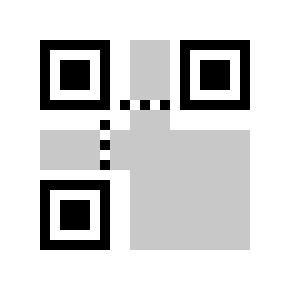
\includegraphics[width=0.145\linewidth]{finder-patterns.png}
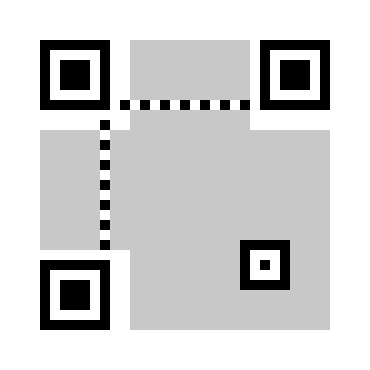
\includegraphics[width=0.185\linewidth]{finder-patterns3.png}
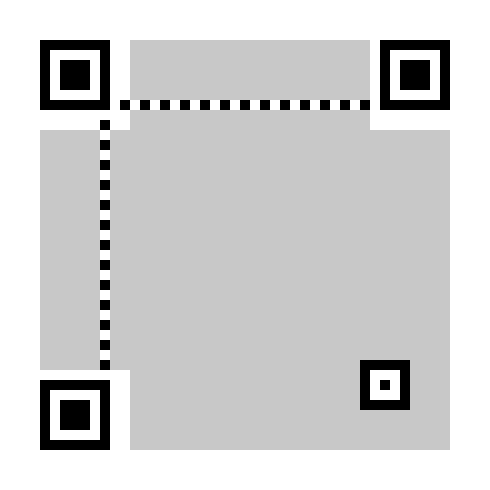
\includegraphics[width=0.245\linewidth]{finder-patterns6.png}\\
Het toevoegen van deze onderdelen heb ik zo geprogrammeerd:
\begin{minted}{python}
class Qr_code:
    ...
    def voeg_finder_en_timing_patterns_toe(self):
        g = self.grootte
        # voeg 'finder patterns' toe
        self.matrix[0:9,0:9] = 0
        self.matrix[0:9,g-8:g] = 0
        self.matrix[g-8:g,0:9] = 0
        for pos in ((0,0),(g-7,0),(0,g-7)):
            self.matrix[pos[0]:pos[0]+7,pos[1]:pos[1]+7] = 1
            self.matrix[pos[0]+1:pos[0]+6,pos[1]+1:pos[1]+6] = 0
            self.matrix[pos[0]+2:pos[0]+5,pos[1]+2:pos[1]+5] = 1
        # `alignment pattern'
        if self.versie>1:
            i = g-7
            self.matrix[i-2:i+3,i-2:i+3] = 1
            self.matrix[i-1:i+2,i-1:i+2] = 0
            self.matrix[(i,i)] = 1
        # voeg `timing patterns' toe (stippellijntjes)
        for i in range(8,g-8,2):
            self.matrix[(i,6)] = self.matrix[(6,i)] = 1
            self.matrix[(i+1,6)] = self.matrix[(6,i+1)] = 0
\end{minted}
Vanaf versie 7 is de opbouw net iets anders. Er zijn dan namelijk extra alignment-patterns en er wordt op twee plaatsen `version information' toegevoegd. Maar omdat die QR-codes minder worden gebruikt, zal ik dat niet uitgebreid behandelen.
\subsubsection{Plaatsing bits in QR-code}
\begin{figure}[h]
\centering
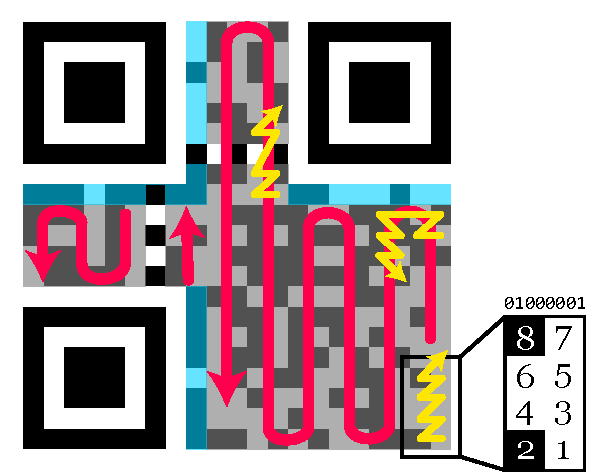
\includegraphics[width=0.7\linewidth]{qr-zigzag.pdf}
\caption{Opbouw QR-code}
\label{fig:zigzag}
\end{figure}
De bits kunnen nu in de QR-code geplaatst worden. Dat gebeurt met een zigzag in een zigzag-patroon. Er wordt rechts-onder begonnen, in de hoek zonder finder-pattern. Een 1 wordt een zwarte module (blokje) en een 0 een witte module.
Figuur \ref{fig:zigzag} laat de plaatsing van de bits zien. Bij de blauwe gebieden moet plaats worden vrijgehouden voor de `format string', die we later toevoegen. De pijlen in de afbeelding geven de volgorde aan waarin de bits in de QR-code gezet moeten worden. Dit waren de bits die we het vorige hoofdstuk hebben berekend:\\\\
\blockms{01000001 00000100 00110110 11110110 01000110 01010111 00100110 10010110 11100110 01110111 00110111 01000110 1000011001010110 11110111 00100110 10010110 01010000 1110110010001000 11100010 10000011 01011000 01010101 11010001 11011010\\}
De eerste bit is een 0, dus in de QR-code wordt rechtsonder een witte module getekend. Daarna komt een 1, dus een zwarte module. Schuin daarboven wordt weer een witte module getekend, en ga zo maar door. Als je bovenaan bent gekomen, ga je in de volgende kolom weer omlaag.

Kom je de timing-pattern tegen (de stippellijntjes), sla je die over en zoek je de eerstvolgende lege plek. In grotere QR-code's moet je ook nog rekening houden met de `aligment pattern'  rechtsonder, net als bij de timing-pattern.
\subsubsection{`Masking'}
\begin{figure}[h]
\centering
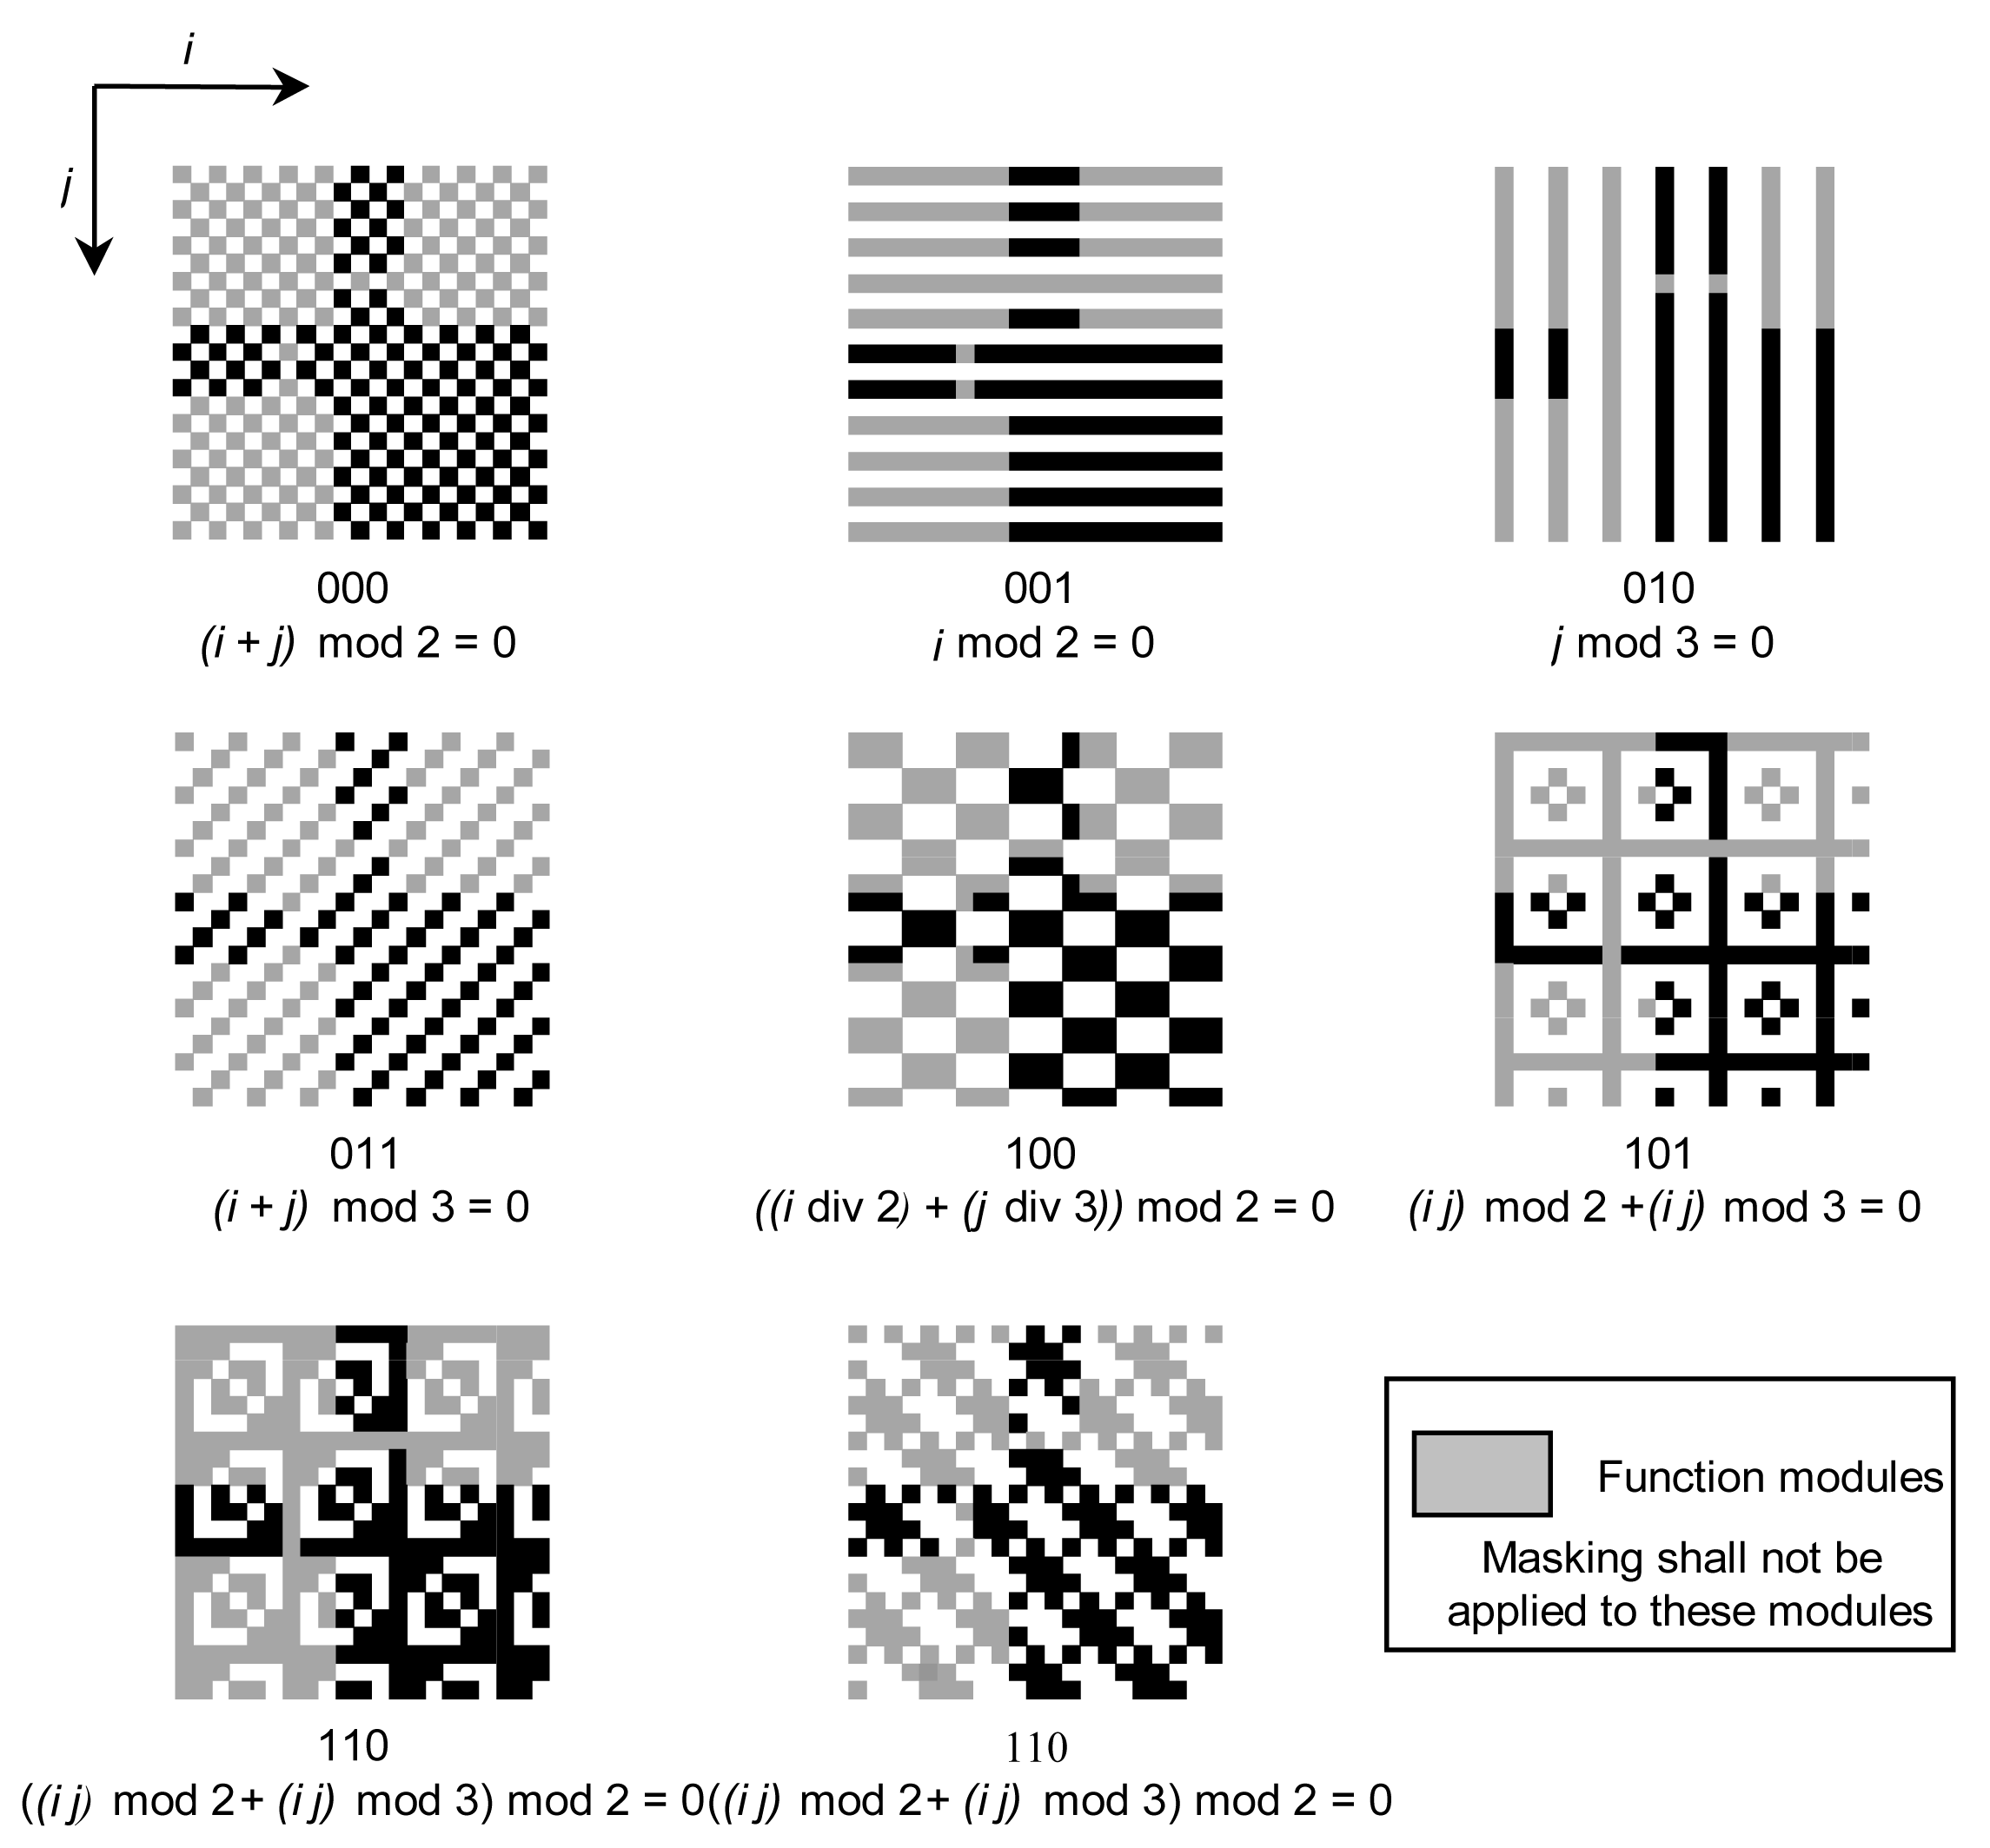
\includegraphics[width=0.8\linewidth]{mask-patterns.png}
\caption{Mask patterns}
\label{fig:mask-patterns}
\end{figure}
De volgende stap is een `mask' toepassen. Dat is nodig voor het scannen. Als er namelijk toevallig in de QR-code ergens de vorm van een finding-pattern ontstaat bij het invullen, zou de scanner van slag kunnen raken. Om dat op te lossen moeten er verschillende patronen `overheen gelegd' worden, en wordt gekozen welke code het best te scannen is.  Figuur \ref{fig:mask-patterns} laat de 8 verschillende patronen zien die gebruikt kunnen worden. Elk patroon wordt gevormd door een bepaalde functie met als argumenten de coördinaten. In de functies wordt modulo 2 of 3 gerekend, waardoor het patroon zich herhaalt. De finder-patterns, de format-string en de alignment-pattern worden niet veranderd door de mask, alleen de inhoud van de QR-code. Is de functie gelijk aan nul op een bepaalde positie, dan moet de de kleur van van de module worden omgedraaid.

Ik heb een functie geprogrammeerd die de QR-code vult, en meteen een mask toepast. Het algoritme om de QR-code te vullen is best ingewikkeld, en het was moeilijk om het te verzinnen. De zessen die je ziet hebben te maken met het feit dat bij de linker timing-pattern een module wordt overgeslagen.
\begin{minted}{python}
class Qr_code:
    ...
    def vul_qr_code(self,qr_bits):
        '''vul de qr-code met bits'''
        # masking formules
        masking = {
            # modulo wordt geschreven als %
            0 : (lambda x,y: (x+y)%2),
            1 : (lambda x,y: y%2),
            2 : (lambda x,y: x%3),
            3 : (lambda x,y: (x+y)%3),
            4 : (lambda x,y: (y/2 + x/3)%2),
            5 : (lambda x,y: (x*y)%2+(x*y)%3),
            6 : (lambda x,y: ((x*y) % 2 + (x*y) % 3) % 2),
            7 : (lambda x,y: ((x*y) % 3 + (x+y) % 2) % 2)
            }
        g = self.grootte
        pos = np.array((g-1,g-1))
        last_bit = len(qr_bits)-1
        for i,bit in enumerate(qr_bits):
            # stel de mask-formule gelijk aan 0
            mask = int(masking[self.mask](pos[0],pos[1]) == 0)
            # verwissel een 1 met een 0 als de vergelijking waar is
            self.matrix[tuple(pos)] = str( mask ^ int(bit) )
            # stop bij de laatste bit
            if i==last_bit:
                break
            # sla de linker timing-pattern over
            if tuple(pos) == (7,9):
                pos += (-2,0)
                continue
            # algoritme voor het zigzag-patroon
            while True:
                dir = 'up'
                if pos[0] < 6 and pos[0] % 4 < 2:
                    dir = 'down'
                if pos[0] > 6 and (pos[0]-1) % 4 < 2:
                    dir = 'down'
                if (pos[0]%2 and pos[0]<6) or (not pos[0]%2 and pos[0]>6):
                    pos += (-1,0)
                # einde van de kolom
                elif (dir=='up' and pos[1]==0) or (dir=='down' and pos[1]==g-1):
                    pos += (-1,0)
                else:
                    pos += (1,(-1 if dir=='up' else 1))
                if self.matrix[tuple(pos)] == -1:
                    # als de module leeg is, zoek dan niet verder
                    break
        # maak overige pixels wit
        for i in range(0,g):
            for j in range(0,g):
                if self.matrix[(i,j)] == -1:
                    self.matrix[(i,j)] = 0 if masking[self.mask](i,j) else 1
\end{minted}
\subsubsection{`Format String'}
\begin{figure}[h]
\centering
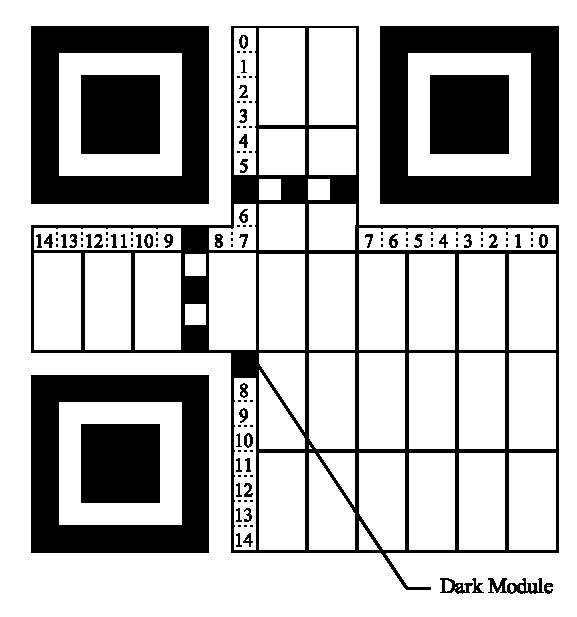
\includegraphics[width=0.5\linewidth]{format-string.pdf}
\caption{Format-string}
\label{fig:format-string}
\end{figure}

De laatste stap is het toevoegen van de format-string, die de gebruikte mask en het e.c-niveau bevat. Deze informatie is met een eenvoudige RS-code gecodeert, en twee keer in de QR-code opgeslagen rondom de drie finder-patterns.

\subsection{Decoderen \& Fouten corrigeren}
\section{Bronvermelding}
\section{Logboek}
\end{document}
